\section{Question 4}

Assume you want to design a classifier which receives univariate data as input and must choose between class $+1$ or class $-1$.
The data associated with class ``$+1$'' follow a gaussian density with mean $2$ and unit variance. 
On the other hand, the data associated with class ``$-1$'' follow a uniform density between $-2$ and $2$. 
The prior probabilities are $P(C_{+1}) = 0.6$ and $P(C_{-1}) = 0.4$.

\subsection{Item a}
Apply Bayes' methodology to obtain the optimal classification model and show, using adiagram, 
the model's architecture (with clear indication of the discriminant function(s)).

\subsection{Item b}
Calculate the model's decision boundary. 
Analytically calculate the classifier error probability (the integrals can be numerically solved).

\subsection{Item c}
Recalculate the model's decision boundary if the Maximum-Likelihood criterion is adopted, this time. 
Analytically calculate the classifier error probability (the integrals can be numerically solved).

\subsection{Item d}
Compare the performances of both methodologies.

\noindent\rule{\textwidth}{.5pt}

A classification model is tasked with assigning a value $x$ on the line as belonging to one of the distributions,
i.e. classifying it as ``$+1$'' or ``$-1$'';
an \textit{optimal} classification model will do so while maximizing its chances/minimizing its error. 

It is given an input $x\in\mathbb{R}$ and 
must output a class $C_B$ such that the conditional probability 
$P(C=C_B|x)$ is the greatest amongst the considered classes.
Using Bayes' theorem, we can write it as
%
\begin{align}
    P(C_B|x) = \frac{p(x|C_B)P(C_B)}{p(x)}
\end{align}
%
with $p(x|C)$, called likelihood, the probability of $x$ happening given that it comes from class $C$.
Since the expression above is valid not only to the optimal choice but for any class, 
and $p(x)$ is invariant with respect to classes, we have 
%
\begin{align}
    C_B 
    = \argmax_C P(C|x)
    = \argmax_C p(x|C)P(C).
\label{eq:max}
\end{align}

Since $x\in\mathbb{R}$, the maximization above splits the real line in compact intervals such that 
$x$ in adjacent intervals result in different $C_B$.
Classification error comes from the true class of a sample not being the class assigned to the associated interval. 

For example, let's say two classes $H_0$ and $H_1$ have likelihoods such that 
the classifier assings $x\in R_0$ to $H_0$ and $x\in R_1$, to $H_1$.
%
Then, the probability of error is given by the integration of 
$P(C=H_1 | x\in R_0)$ plus the integration of 
$P(C=H_0 | x\in R_1)$, i.e., the proportion of false negatives and positives with respect to $H_1$:
%
\begin{align}
    P_\text{error} 
    &= P(H_1 | x\in R_0) + P(H_0 | x \in R_1)
    \\
    &= 
    P(H_1) \int_{R_0} p(x | H_1)\ dx +
    P(H_0) \int_{R_1} p(x | H_0)\ dx.
\label{eq:error}
\end{align}

Had we begun this answer by assuming a classifier maps regions 
$R_0$, $R_1$ to classes, the optimal classifier would minimize $P_\text{error}$ 
by picking looking at the values of $P(H_i)p(x|H_i)$ and chossing $H_i$ with biggest result.

Let's finally apply this Bayesian approach to the problem in question.
Since there are two classes and one of them is gaussian, 
it is useful to rewrite the maximization problem in \eqref{eq:max} as 
%
\begin{align}
    C_B = 
    \begin{cases}
        C_{+1}, & g(x) > 0 \\
        C_{-1}, & g(x) < 0
    \end{cases},
    \quad
    g(x) = g_B(x) =
    \ln \frac{p(x|C_{+1}) P(C_{+1})}
              {p(x|C_{-1}) P(C_{-1})}
\end{align}

The function $g_B$, the discriminant of the classifier, is explicitly given by 
%
\begin{align}
    g_B(x)
    &=
    \ln \frac{p(x|C_{+1}) P(C_{+1})}
              {p(x|C_{-1}) P(C_{-1})} \\
    &=
    \ln[p(x|C_{+1})] + \ln[P(C_{+1})]
    -\ln[p(x|C_{-1})] - \ln[P(C_{-1})] \\
    &=
    \begin{cases}
        -\frac{1}{2}\ln(2\pi) -\frac{1}{2}(x-2)^2 + \ln(0.6) 
        - \ln(1/4) - \ln(0.4), & |x|\leq 2 \\ 
        \infty, & |x| > 2 
    \end{cases}
\label{eq:discriminant}
\end{align}

where it was used the fact that 
$P(C_{+1}) = 0.6$, 
$P(C_{-1}) = 0.4$, 
$p(x|C_{+1}) = \frac{1}{\sqrt{2\pi}} e^{-\frac{1}{2}(x-2)^2}$, and
$P(x|C_{-1}) = 1/4$, if $|x|\leq 2$, and 
$P(x|C_{-1}) = 0$, otherwise.
%
From \eqref{eq:discriminant}, one can deduce that the classifier decision boundary, i.e., the roots of the discriminant,
is a single point $\delta_B = 2-\sqrt{\ln(36/2\pi)}$; 
$x > \delta_B$ or $x < -2$ are classified as $C_{+1}$, and 
$-2 < x < \delta_B$ are classified as $C_{-1}$.

On $|x|\leq 2$, the error probability of this classifier can be calculated using \eqref{eq:error}:
%
\begin{align}
    P^B_\text{error} 
    = 
    0.6 
    \int_{-2}^{\delta_B} \frac{1}{\sqrt{2\pi}} e^{-\frac{1}{2}(x-2)^2}\ dx
    +
    0.4 
    \int_{\delta_B}^2 \frac{1}{4}\ dx
    =
    0.1880\dots
\end{align}

As commented, this classifier minimizes the probability of error.
If a different discriminant was used, such as Maximum-Likelihood (ML) criterion, error would increase.
Indeed, taking
%
\begin{equation}
    g(x) = g_\text{ML}(x)
    =
    \ln \frac{p(x|C_{+1})}
              {p(x|C_{-1})}
    =
    \begin{cases}
        -\frac{1}{2}\ln(2\pi) -\frac{1}{2}(x-2)^2  
        - \ln(1/4), & |x|\leq 2 \\ 
        \infty, & |x| > 2 
    \end{cases}
\end{equation}
%
nudges the threshold to $\delta_\text{ML} = 2-\sqrt{\ln(16/2\pi)}$ and result in sligthly higher error probability:
%
\begin{align}
    P^\text{ML}_\text{error} 
    = 
    0.6 
    \int_{-2}^{\delta_\text{ML}} \frac{1}{\sqrt{2\pi}} e^{-\frac{1}{2}(x-2)^2}\ dx
    +
    0.4 
    \int_{\delta_\text{ML}}^2 \frac{1}{4}\ dx
    =
    0.1967\dots
\end{align}

\Cref{fig:distributions} shows the problem with choosing ML over the Bayesian approach:
while both methods try to place a boundary between classes by looking at their likelihoods,
ML ignores priors, skewing its perception of data. 
Had the priors been equal, however, ML would be identical to the optimal classifier. 
In general, the more variance between classes priors, the worse ML performs.
%
\begin{figure}[hbp]
    \centering 
    \caption{Class conditional distributions before and after being weighted by their priors.}
    \label{fig:distributions}
    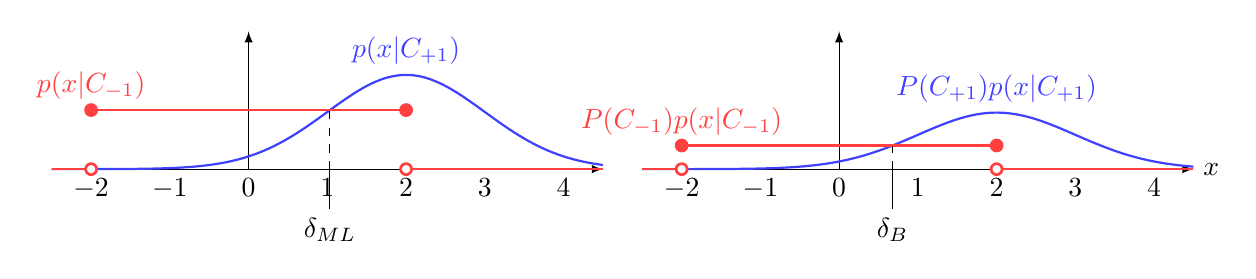
\begin{tikzpicture}[> = latex, domain=-2.5:4.5, samples=100]
    \def\r{1.75 * 0.05}
    \def\yScale{3}
    % Distributions before priors: Maximum-Likelihood estimator
    % Axis
    \draw [->] (-2.5, 0) -- (4.5, 0);
    \draw [->] (0, 0) -- (0, 1.75);
    \foreach \x in {-2, -1, 0, 1, 2, 3, 4}{
        \draw (\x, 0) node [below] {$\x$};
    }
    % p(x|C+1)
    \draw [thick, blue!75] 
        plot (\x, {\yScale * 0.39894 * exp(-0.5 * (\x-2) * (\x-2))})
        (2, \yScale * 0.39894) node [above] {$p(x|C_{+1})$};
    % p(x|C-1)
    \def\deltaML{1.033} % 
    \draw [thick, red!75] 
        (-2, \yScale * 1/4) node [above] {$p(x|C_{-1})$} --++ (4, 0)
        (2, 0) -- (4.5, 0)
        (-2, 0) -- (-2.5, 0)
    ;
    \fill [red!75]
        (-2, \yScale * 1/4) circle (\r)
        (2, \yScale * 1/4) circle (\r)
        (-2, 0) circle (\r)
        (2, 0) circle (\r)
    ;
    \fill [white]
        (-2, 0) circle (\r-1.75 * 0.02)
        (2, 0) circle (\r-1.75 * 0.02)
    ;
    \draw (\deltaML, 0) --++ (0, -0.5) node [below] {$\delta_\text{ML}$};
    \draw [dashed] (\deltaML, 0) --++ (0, \yScale * 1/4);

    % Distributions after priors: Bayes estimator (optimal)
    \def\deltaB{0.67877} % 
    \def\priorOne{0.6}
    \def\priorMinusOne{0.4}
    \begin{scope}[shift={(7.5, 0)}]
        % Axis
        \draw [->] (-2.5, 0) -- (4.5, 0) node [right] {$x$};
        \draw [->] (0, 0) -- (0, 1.75);
        \foreach \x in {-2, -1, 0, 1, 2, 3, 4}{
            \draw (\x, 0) node [below] {$\x$};
        }
        % p(x|C+1)
        \draw [thick, blue!75] 
            plot (\x, {\yScale * \priorOne * 0.39894 * exp(-0.5 * (\x-2) * (\x-2))})
            (2, \yScale * \priorOne * 0.39894) node [above] {$P(C_{+1}) p(x|C_{+1})$};
        % p(x|C-1)
        \draw [thick, red!75] 
            (-2, \yScale * \priorMinusOne * 1/4) node [above] {$P(C_{-1}) p(x|C_{-1})$} --++ (4, 0)
            (2, 0) -- (4.5, 0)
            (-2, 0) -- (-2.5, 0)
        ;
        \fill [red!75]
            (-2, \yScale * \priorMinusOne * 1/4) circle (\r)
            (2, \yScale * \priorMinusOne * 1/4) circle (\r)
            (-2, 0) circle (\r)
            (2, 0) circle (\r)
        ;
        \fill [white]
            (-2, 0) circle (\r-1.75 * 0.02)
            (2, 0) circle (\r-1.75 * 0.02)
        ;
        \draw (\deltaB, 0) --++ (0, -0.5) node [below] {$\delta_\text{B}$};
        \draw [dashed] (\deltaB, 0) --++ (0, \yScale * \priorMinusOne * 1/4);
    \end{scope}
\end{tikzpicture}
\end{figure}
%